\section{Auswertung}
\label{sec:Auswertung}
Um die Messwert auswerten zu können, ist es erforderlich,
dass zunächst der Dopplerwinkel \alpha der drei Prismenwinkel \theta
mit Hilfe der Formel \eqref{eqn:prism} berechnet wird.
Die Dopplerwinkel zu den entsprechenden Prismenwinkel
sind in der Tabelle \ref{tab:winkel} zu finden.
\begin{table}
  \centering
  \caption{Prismen- und Dopplerwinkel.}
  \label{tab:winkel}
  \begin{tabular}{c c c}
    \toprule
    Prismenwinkel $\theta/\si{\degree}$& Dopplerwinkel $\alpha / \si{\degree}$& Dopplerwinkel $\alpha /\si{\radian}$\\
    \midrule
15 & 80,064 & 1.397\\
30 & 70,529 & 1.231\\
60 & 54,786 & 0.956\\
    \bottomrule
  \end{tabular}
\end{table}
\subsection{Messung 1}
Die Messwerte, die durch die im Kapitel \ref{sec:durchführung} beschriebenen Methode
aufgenommen werden, sind in der Tabelle \ref{tab:mess1} aufgelistet.
\begin{table}
  \centering
  \caption{Messwerte der Geschwindigkeit $v$ und $\Delta\nu$ für unterschiedliche Winkel.}
  \label{tab:mess1}
  \begin{tabular}{c c c c c c}
    \toprule
    \multicolumn{2}{c}{ $\theta=15\si{\degree}$ } &  \multicolumn{2}{c}{ $\theta=30\si{\degree}$ } & \multicolumn{2}{c}{ $\theta=60\si{\degree}$ } \\
    $v/\si{\meter\per\second}\cdot10^{-3}$ & $\Delta\nu/\si{\hertz}$ & $v/\si{\meter\per\second}\cdot10^{-3}$ & $\Delta\nu/\si{\hertz}$ & $v/\si{\meter\per\second}\cdot10^{-3}$ & $\Delta\nu/\si{\hertz}$ \\
    \midrule
    19,1  & 673  & 13,2  & 98  & 8,6  & 110\\
    66,8  & 6256 & 48,6  & 360 & 26,6 & 342\\
    132,1 & 6507 & 93,1  & 690 & 47,6 & 610\\
    154,3 & 6592 & 119,5 & 885 & 51,9 & 665\\
    140   & 6537 & 123,6 & 916 & 58,5 & 751\\
    \bottomrule
  \end{tabular}
\end{table}
\FloatBarrier
Diese werden nun in der Form $\Delta\nu/\cos\alpha$ in Abhängigkeit von der Geschwindigkeit $v$, wie in der Abbildung \ref{fig:mess1} zu sehen, aufgetragen.
Ebenfalls enthält die Abbildung \ref{fig:mess1} eine Gerade, die sich durch umstellen der Theoretische Formel \eqref{eqn:deltav} in die Form
\begin{align}
  \frac{\Delta\nu}{\cos{\alpha}}=2\nu_0\cdot\frac{v}{c}.\label{eqn:theo}
\end{align}
ergibt. Das c in der Formel ist die Schallgeschwindkeit ( im  Medium) (Luft), die genau
\begin{align}
  c=??.
\end{align}
beträgt. Die Frequenz der Ultraschallquelle $\nu_0$ beträt hier:
\begin{align}
  \nu_0=2\si{\mega\hertz}.
\end{align}
\FloatBarrier
\begin{figure}
  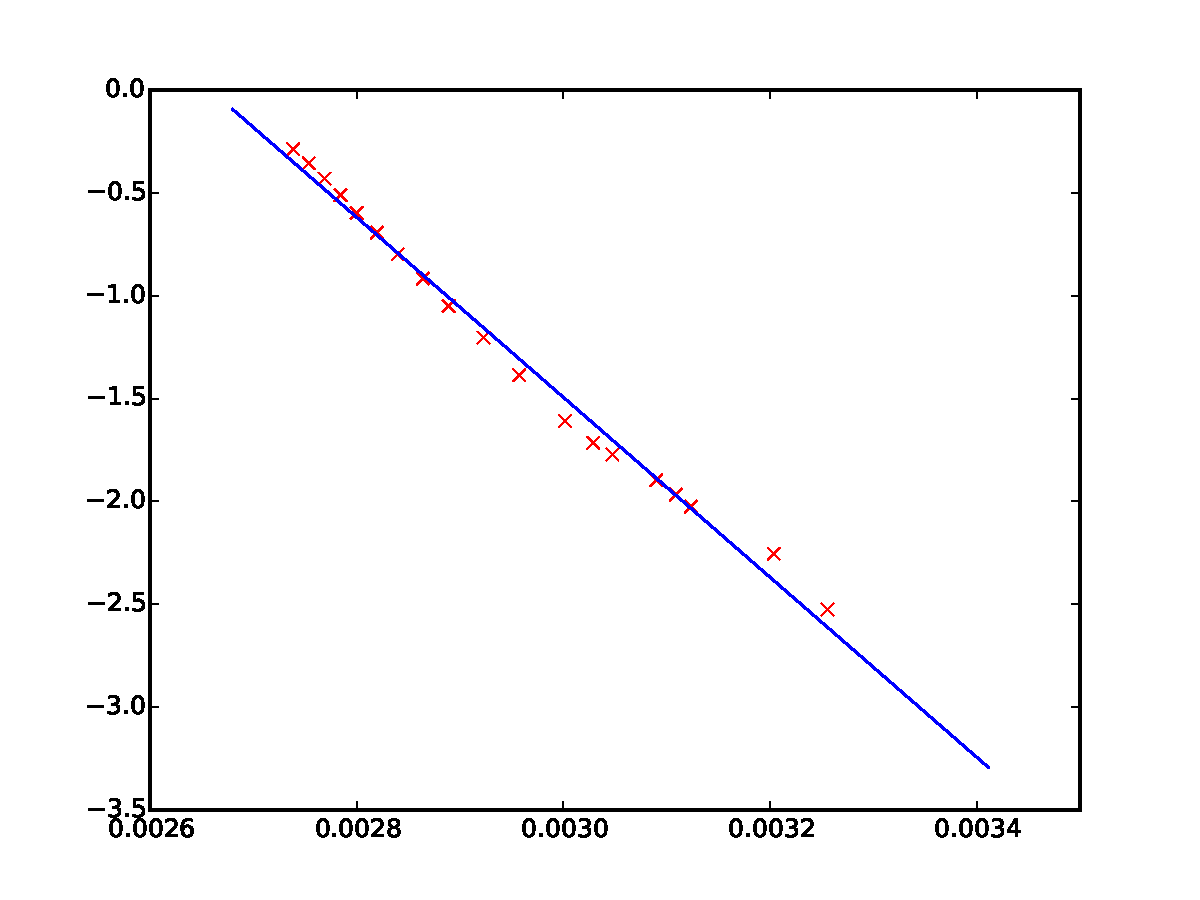
\includegraphics[width=0.7\textwidth]{plot1.pdf}
  \centering
   \caption{$\Delta\nu/\cos\alpha$ in Abhängigkeit von der Geschwindigkeit $v$ für die Messwerte aus der Tabelle \ref{tab:mess1} und für die theorietische Formel \eqref{eqn:theo}.}
  \label{fig:plot}
\end{figure}

\newpage
\subsection{Messung 2}
Die Werte der gemessenen Strömungsprofile des $3/8$ Zoll Schlauches bei einem Winkel
$\theta$ von $15\si{\degree}$ für eine Strömungsleistung von 40 und 60 Prozent sind in der Tabelle \ref{tab:mess2}
aufgelistelt.
\begin{table}
  \centering
  \caption{Messwerte der Geschwindigkeit $v$ und der Streuintensität $\beta$ bei unterschiedlichen Eindringtiefe $s$.}
  \label{tab:mess2}
  \begin{tabular}{c c c c c}
    \toprule
       & \multicolumn{2}{c}{ $60\%$ Strömungsleistung } &  \multicolumn{2}{c}{$40\%$ Strömungsleistung  } \\
     $s/\si{\meter}\cdot10^{-3}$ & $v/\si{\meter\per\second}\cdot10^{-3}$ & $\beta/1000\si{\volt\tothe{2}\per\second} $ & $v/\si{\meter\per\second}\cdot10^{-3}$ &$\beta/1000\si{\volt\tothe{2}\per\second}$ \\
     \midrule
     0     & 25,5 & 70  & 15,9 & 14\\
     0,75  & 22,3 & 161 & 12,7 & 83\\
     1,5   & 25,5 & 100 & 14,3 & 258\\
     2,25  & 22,3 & 61  & 15,9 & 367\\
     3,0   & 27,0 & 81  & 15,9 & 735\\
     3,75  & 28,6 & 61  & 15,9 & 817\\
     4,5   & 28,6 & 47  & 15,9 & 438\\
     5,25  & 28,6 & 12  & 19,1 & 364\\
     6,0   & 33,4 & 10  & 19,1 & 359\\
     6,75  & 35,0 & 8   & 19,1 & 252\\
     7,5   & 35,0 & 9   & 22,3 & 202\\
     8,25  & 31,8 & 9   & 22,3 & 147\\
     9,0   & 35,0 & 8   & 22,3 & 140\\
     9,75  & 31,8 & 9   & 22,3 & 109\\
     10,5  & 36,6 & 8   & 22,3 & 84\\
    \bottomrule
  \end{tabular}
\end{table}
\FloatBarrier
Nun wird einmal die Strömungsgeschwindigkeit $v$ in Abbildung \ref{fig:v2} sowie die Streuintensität
$\beta$ in Abbildung \ref{fig:b2} in Abhängikeit der Eindringtiefe $s$ aufgetragen.
\begin{figure}
  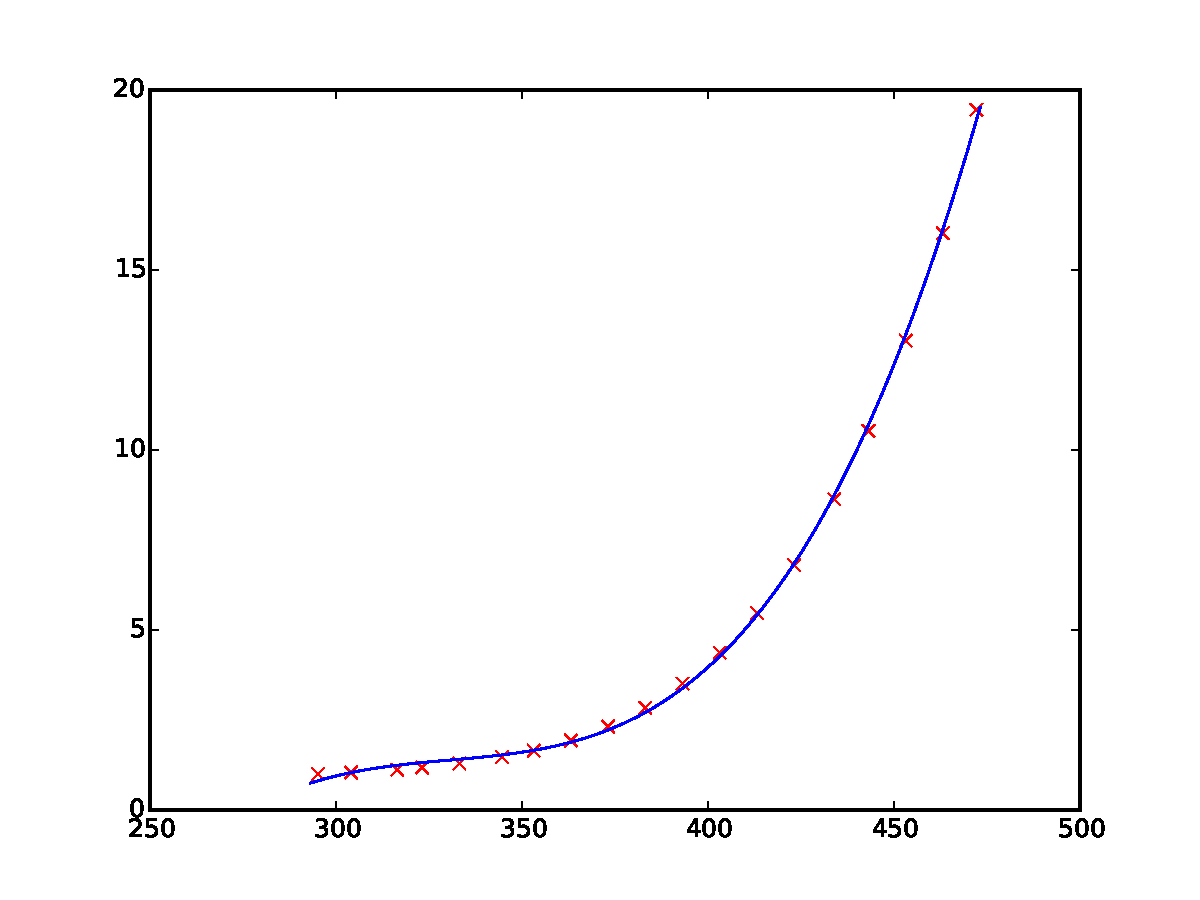
\includegraphics[width=0.7\textwidth]{plot2.pdf}
  \centering
   \caption{Die Geschwindigkeit $v$ in Abhängigkeit von der Eindringtiefe $s$ für die Messwerte aus der Tabelle \ref{tab:mess2}.}
  \label{fig:v2}
\end{figure}

\begin{figure}
  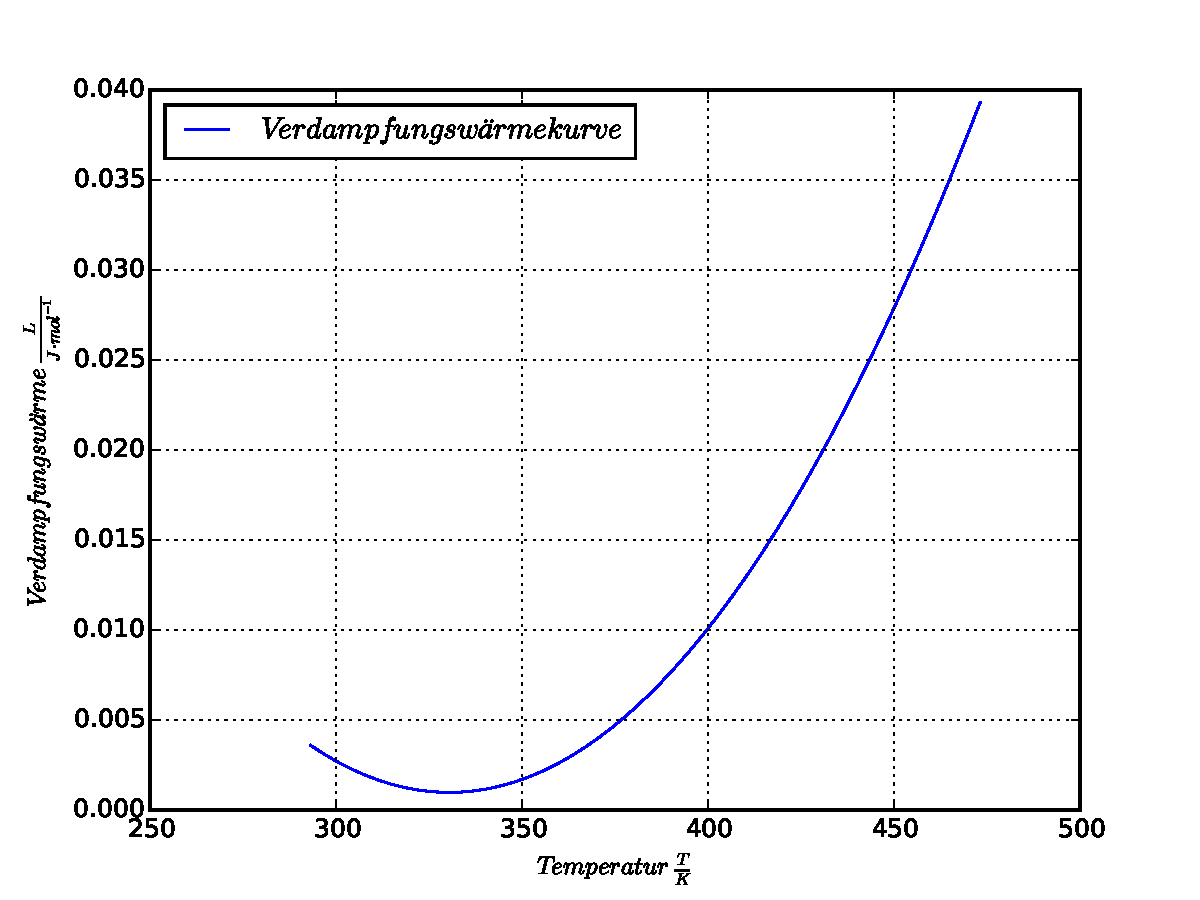
\includegraphics[width=0.7\textwidth]{plot3.pdf}
  \centering
   \caption{Die Streuintensität $\beta$ in Abhängigkeit von der Eindringtiefe $s$ für die Messwerte aus der Tabelle \ref{tab:mess2}.}
  \label{fig:b2}
\end{figure}
